%% Author: 	Aaron <azet@azet.org> Zauner
%% License:	https://creativecommons.org/licenses/by-nc-nd/4.0/

%% theme and colorscheme
\documentclass[hyperref={draft}]{beamer}
\usecolortheme[dark,accent=white]{solarized}
\beamertemplatetransparentcovered
\setbeamertemplate{navigation symbols}{}

%% packages
\usepackage[light,math]{iwona}
\usepackage[T1]{fontenc}
\usepackage{textpos}
\usepackage{tikz}
\usepackage{mathtools}
\usepackage{appendixnumberbeamer} 
\usepackage{listings}
\usepackage{anyfontsize}

%% footer
\setbeamertemplate{footline}[text line]{%
  \parbox{\linewidth}{\vspace*{-15pt}
		      \insertdate \hfill \inserttitle \newline
		      \insertshortauthor \hfill \insertframenumber/\inserttotalframenumber
		     }}
\setbeamertemplate{navigation symbols}{}

%% title
\title{Introduction to and survey of TLS Security}
%\subtitle{Introduction and Survey}

%% author and affilliation
\author[Aaron Zauner]{Aaron Zauner\\
	      \textit{azet@azet.org}\\
	      
\includegraphics[height=65px,width=65px]{lambda}
       }
\institute{lambda.co.at:\\Highly-Available, Scalable \& Secure Distributed Systems}

%% venue and date
\date{BsidesHH - 28/12/2014}

%%
%% main
%%
\begin{document}

{
\setbeamertemplate{footline}{} 

\begin{frame}
  \titlepage
\end{frame}

}
\addtocounter{framenumber}{-1}

{
\setbeamertemplate{footline}{}

\begin{frame}{Table of Contents}
  \tableofcontents
\end{frame}

}
\addtocounter{framenumber}{-1}


\addtobeamertemplate{frametitle}{}{%
  \begin{tikzpicture}[remember picture,overlay]
    \node[anchor=north east,yshift=1pt] at (current page.north east) {
      
\includegraphics[height=30px]{lambda}
    };
  \end{tikzpicture}
}


\section{Motivation}

\begin{frame}{Motivation}
  TLS is something we deal with on a daily basis, so this is an obvious topic for education.
  \newline
  \newline
  Keep in mind that these attacks are not only possible for nation-state actors, some of them I can mount on this very laptop.
\end{frame}

\begin{frame}{Motivation}
    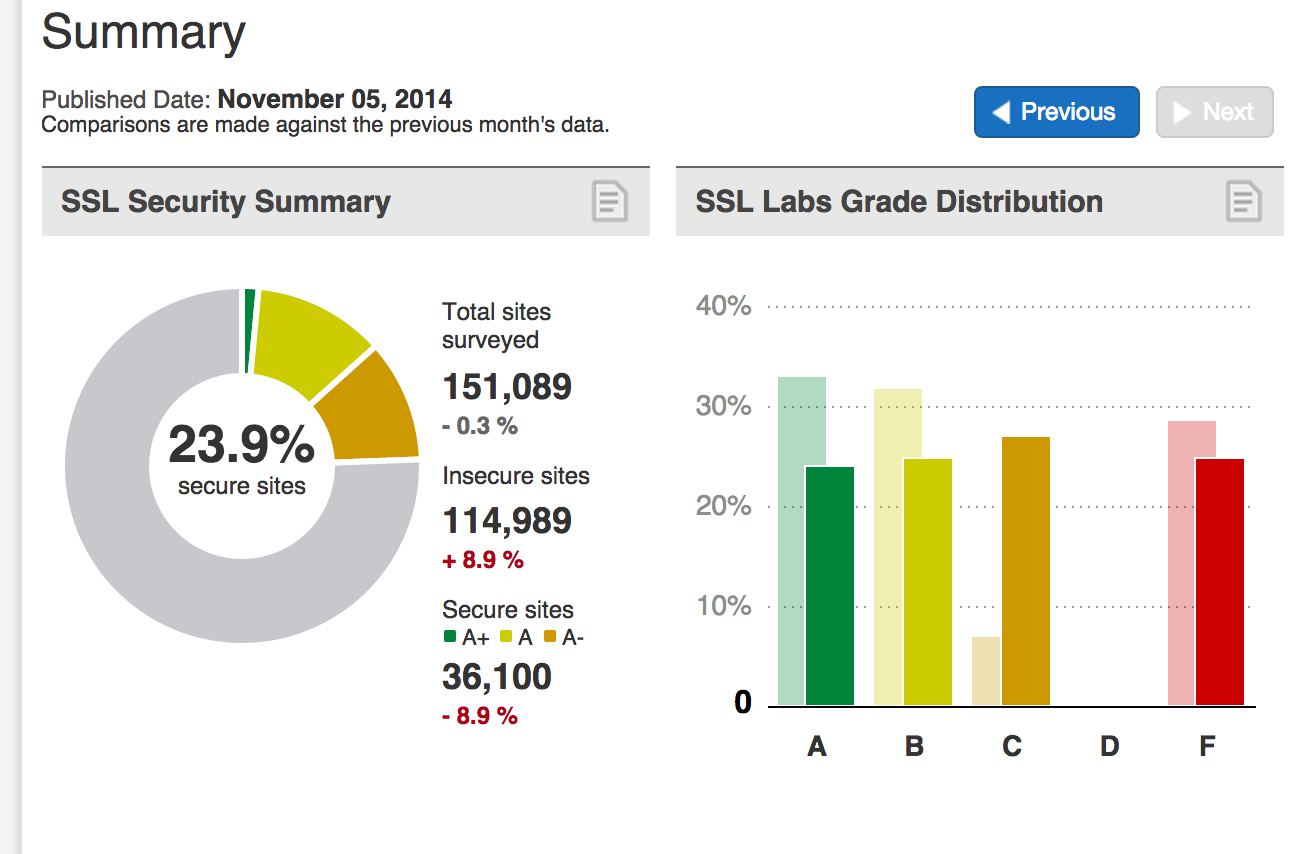
\includegraphics[height=180px]{sslpulse1}

    \vspace{10px}

    \tiny
    \url{https://www.trustworthyinternet.org/ssl-pulse}
\end{frame}


\begin{frame}{Motivation}
    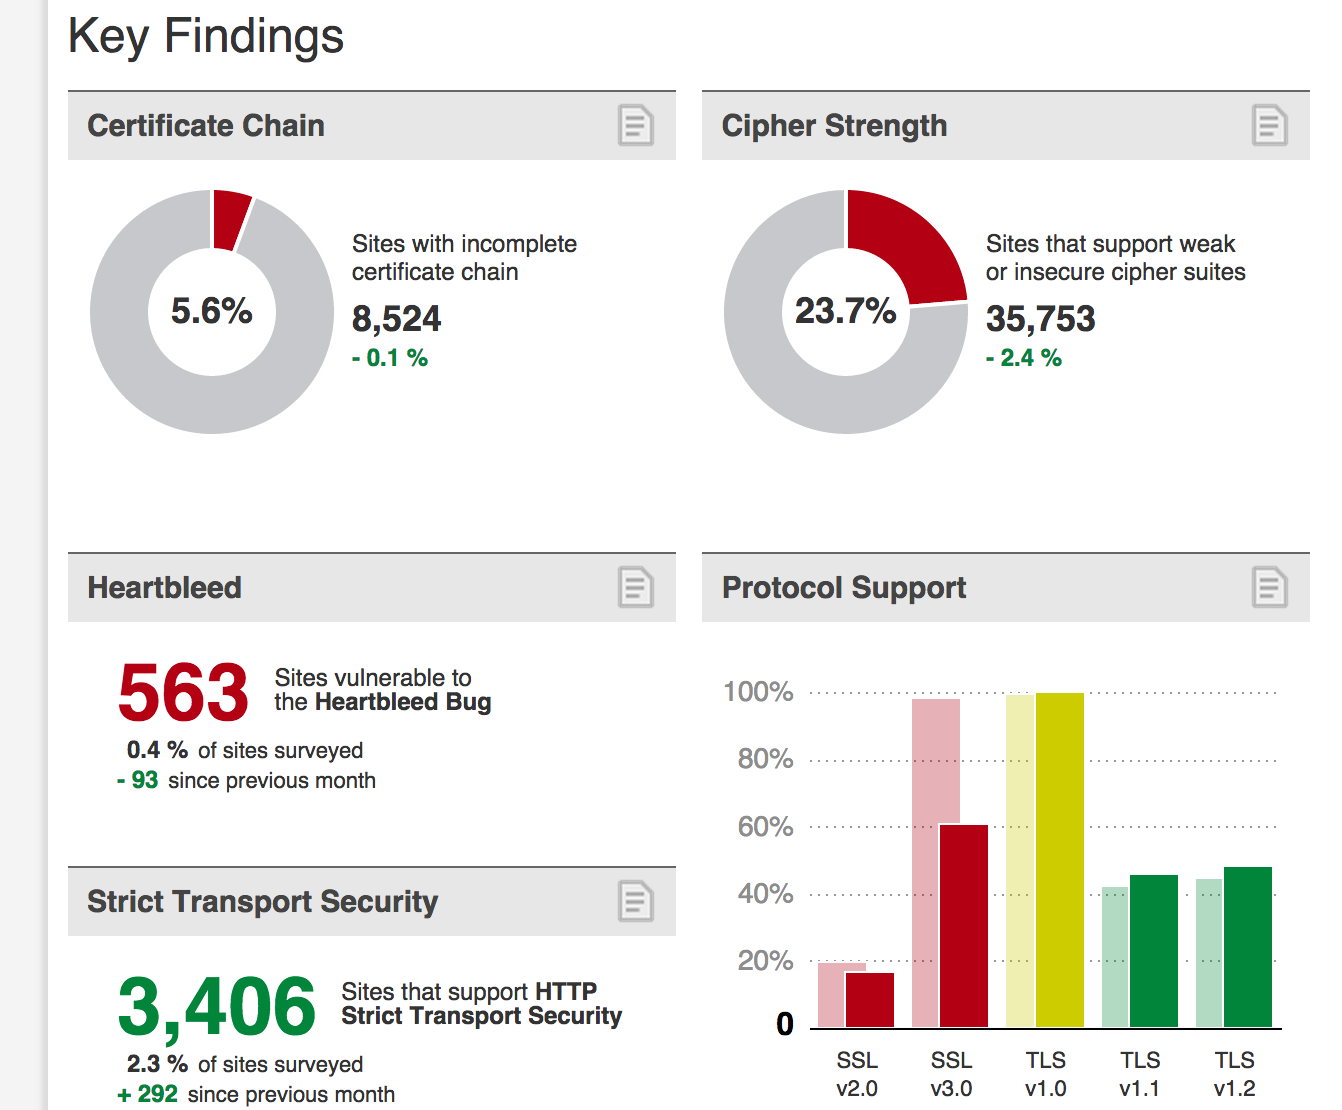
\includegraphics[height=180px]{sslpulse2}

    \vspace{10px}

    \tiny
    \url{https://www.trustworthyinternet.org/ssl-pulse}
\end{frame}
\begin{frame}{Motivation}
    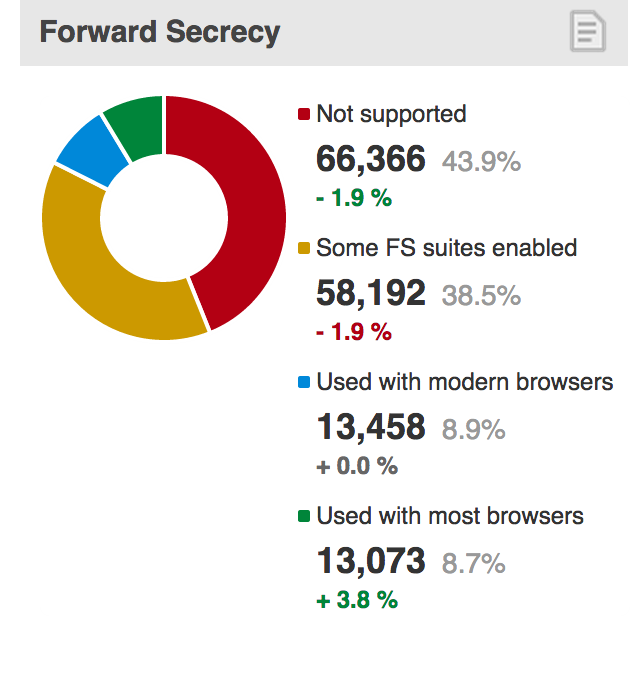
\includegraphics[height=180px]{sslpulse3}

    \vspace{10px}

    \tiny
    \url{https://www.trustworthyinternet.org/ssl-pulse}
\end{frame}
\begin{frame}{Motivation}
    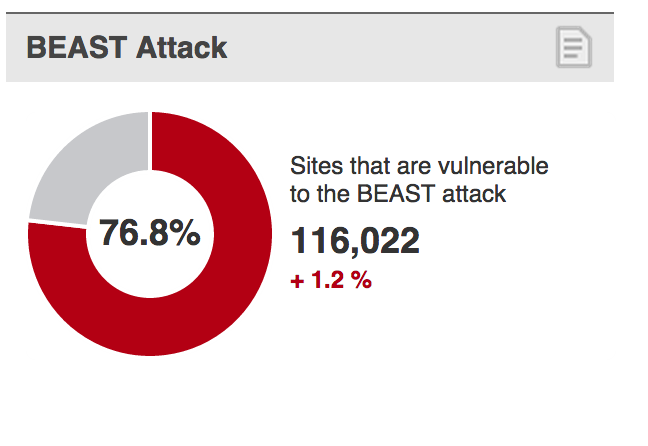
\includegraphics[height=120px]{sslpulse4}

    \vspace{10px}

    \tiny
    \url{https://www.trustworthyinternet.org/ssl-pulse}
\end{frame}


\section{Background}


\subsection{Information Security and Cryptography}

\begin{frame}{Background}
  \framesubtitle{Disclaimer}
  Unfortunately this is not a talk about InfoSec nor cryptography, so I will only cover the very basics needed to understand the topic properly. Background information on Information Security and Cryptography herein is fitted to TLS only.
  \newline
  \newline
  I will recommend appropriate resources for those who want to gain a deeper understanding at the end of my talk.
\end{frame}

\begin{frame}{Background}
  \framesubtitle{Basics}
  Information Security mandates at minimum the following three properties in a secure protocol:
  \begin{itemize}
    \item \textbf{C}onfidentiality
    \item \textbf{I}ntegrity
    \item \textbf{A}vailability (discussed later)
  \end{itemize}
  ..this is commonly known as the ``CIA triad'' (seriously). You will see later on why these are paramount. The triad is usually extended by:
  \begin{itemize}
    \item Authenticity \& Non-repudiation
  \end{itemize}
\end{frame}

\begin{frame}{Background}
  \framesubtitle{Confidentiallity}
  \begin{itemize}
    \item Prevent unauthorized disclosure of information
    \item \emph{Encryption} and \emph{Decryption} of confidential data
  \end{itemize}
  Example: Rijndael cipher. Later renamed AES (Advanced Encryption Standard) after winning a NIST challenge by the same name.
  \begin{itemize}
    \item Symmetric 128, 192 or 256 bit \textbf{block cipher} 
    \item Stick figure guide to AES: \url{http://www.moserware.com/2009/09/stick-figure-guide-to-advanced.html}
  \end{itemize}
\end{frame}

\begin{frame}{Background}
  \framesubtitle{Confidentiallity: Block cipher modes}
  Block ciphers operate on fixed size \emph{blocks of data}.\\
  Online communication is defined by \emph{streams of data}.
  \newline
  \newline
  Block cipher modes repeatedly apply a given cipher to a stream of data.
  Examples include:
  \begin{itemize}
    \item Cipher-Block Chaining Mode (CBC)
    \item Counter Mode (CTR)
    \item Galois-Counter Mode (GCM) \textbf{[authenticated]}
    \item Counter with CBC-MAC (CCM) \textbf{[authenticated]}
    \item Offset Codebook Mode (OCB) \textbf{[authenticated]}
  \end{itemize}
\end{frame}

\begin{frame}{Background}
  \framesubtitle{Confidentiallity: Block cipher modes}
  \begin{itemize}
    \item CBC Mode (sequential):\\
    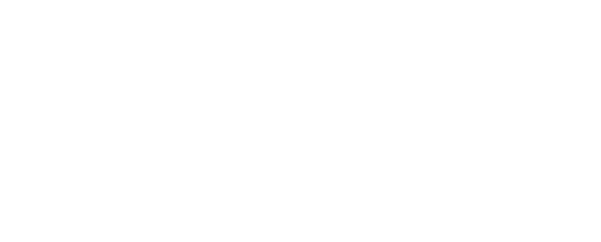
\includegraphics[height=80px]{CBC_encryption}\\
    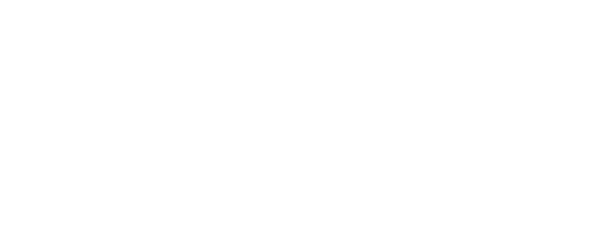
\includegraphics[height=80px]{CBC_decryption}
  \end{itemize}
\end{frame}

\begin{frame}{Background}
  \framesubtitle{Confidentiallity: Block cipher modes}
  \begin{itemize}
    \item CTR Mode (parallel):\\
    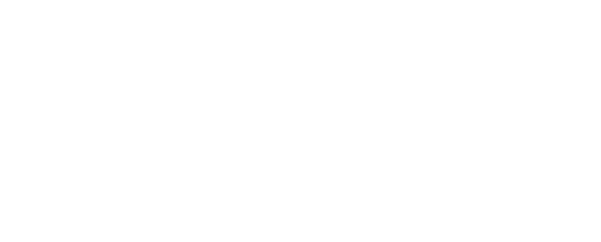
\includegraphics[height=80px]{CTR_encryption}\\
    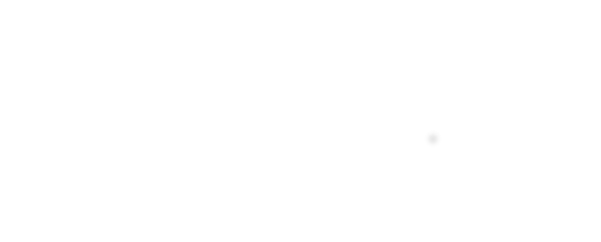
\includegraphics[height=80px]{CTR_decryption}
  \end{itemize}
\end{frame}

\begin{frame}{Background}
  \framesubtitle{Integrity}
  \begin{itemize}
    \item Assures consistency of data
    \item e.g. tampered data will be detected (and may be discarded)
    \item Cryptographic hash functions like SHA can provide integrity by acting as a Hash based Message Authentication Code (HMAC) on the message to be sent and recieved
    \item Hash-functions need to be collission-resistant: Two different inputs should never produce the same hash!
    \item Ideally messages should be encrypted first then MACed (encrypt-then-mac, ETM) to prevent against attacks (CCA, CPA) and to provide for integrity of ciphertexts and plaintexts.\\
    See: \url{http://bit.ly/1kZA6WR}
    \item Authenticated Encryption with Associated Data (AEAD) can be used instead (e.g. GCM, CCM, OCB)
  \end{itemize}
\end{frame}

\begin{frame}{Background}
  \framesubtitle{Authenticity \& Non-repudiation}
  \begin{itemize}
    \item Assures that the involved parties are genuine
    \item i.e. are who they say they are
    \begin{itemize}
      \item Injection attacks
      \item Man-In-The-Middle (MITM) attacks
      \item Various cryptographic attack vectors
    \end{itemize}
  \end{itemize}
  Examples:
  \begin{itemize}
    \item RSA (Rivest, Shamir, Adleman)
    \item DSA (Digital Signature Algorithm)
    \item ECDSA (Elliptic Curve DSA)
    \item Ed25519 (\url{http://ed25519.cr.yp.to})
    \item ElGamal Signature System
  \end{itemize}
\end{frame}

\begin{frame}{Background}
  \framesubtitle{Authenticity \& Non-repudiation: RSA}
  RSA
  \begin{itemize}
    \item Used for:
    \begin{itemize}
      \item Signatures
      \item Certificates
      \item Authenticated Key-Exchanges (don't)
      \item Encryption
    \end{itemize}
    \item Security based on the difficulty of factoring integers:
    \begin{itemize}
      \item $p, q$ are large prime numbers (e.g. $\approx 1024 \text{bits}$)
      \item $N = p \times q$
      \item find factors of $N$
    \end{itemize}
    \item Best known algorithm ($\sim$1994): General Number Field Sieve
    \item Computational complexity for $n$-bits: $O\Big(\exp\big(( \frac{64}{9}n )^\frac{1}{3} ( \log{n} )^\frac{2}{3}\big)\Big)$
  \end{itemize}
\end{frame}

\begin{frame}{Background}
  \framesubtitle{Authenticity \& Non-repudiation: RSA}
  RSA Key Generation
  \begin{itemize}
    %\item Alice chooses two large primes $p$ and $q$ and computes:
    %\item $N = p \times q$
    \item integer $N$ is the product of two large primes $p$ and $q$
    \item $\phi(N) = (p-1)(q-1)$ 
    \item choose an integer $e$ (usually \emph{65537}), such that
    \begin{itemize}
      \item $1 < e < \phi(N)$
      \item $\gcd(e, \phi(N)) = 1$
    \end{itemize}
    \item Public Key: $N$ \emph{(modulus)}, $e$ \emph{(public exponent)}
    \item Private Key: $d \equiv e^{-1} \pmod{\phi(N)}$
  \end{itemize}
  \vspace{30px}
  \tiny$\gcd$ and $\phi$ denote the \emph{Greatest Common Divisor (Euclidian algorithm)} and \emph{Euler totient function}, respectively.
  \newline
  \newline
  Math background: \emph{Modular arithmetic}.\\
  Proof: \emph{Euler's theorem} and \emph{Fermat's little theorem}.
\end{frame}

\begin{frame}{Background}
  \framesubtitle{Authenticity \& Non-repudiation: RSA}
  Alice sends her public key (modulus $N$ and exponent $e$) to Bob\\
  Bob sends his public key (modulus $N$ and exponent $e$) to Alice
  \vspace{10px}
  \begin{columns}[T]
    \column{.5\textwidth}
    RSA Encryption:
    \begin{itemize}
      \item Bob wants to send a message $M$ to Alice, turns $M$ into an integer $m$ ($0 \leq m < N$) using a common padding-scheme
      \item ..computes ciphertext\\ $c \equiv m^e \pmod N$
    \end{itemize}
    \column{.5\textwidth}
    RSA Decryption:
    \begin{itemize}
      \item Bob sends ciphertext to Alice
      \item Alice computes\\$m \equiv c^d \pmod N$
      \item ..recoveres Bob's message $M$ by reversing the common padding-scheme
    \end{itemize}
  \end{columns}
\end{frame}

\begin{frame}{Background}
  \framesubtitle{Authenticity \& Non-repudiation: RSA padding}
  ..a secure padding scheme is really important.

  \vspace{20px}
 
  Example: Bleichenbacher attack on PKCS\#1\\
  \url{http://tinyurl.com/bleichenbacher} (real world SSLv3 attack)
  
  \vspace{20px}

  Not going into that here has been explained in detail in a 31c3 talk yesterday, see also: \url{http://tinyurl.com/rsa-padding}
\end{frame}

\begin{frame}{Background}
  \framesubtitle{Key Agreement}
  A key exchange algorithm exchanges cryptographic keys (i.e. shared secrets) among parties which want to communicate confidentialy.
\end{frame}

\begin{frame}{Background}
  \framesubtitle{Key Agreement: Diffie-Hellman}
  The Diffie-Hellman key exchange algorithm (1976) was the first scheme devised to exchange cryptographic keys among multiple parties. It is the most widely used key exchange algorithm to this date.
\end{frame}

\begin{frame}{Background}
  \framesubtitle{Key Agreement: Diffie-Hellman}
  Alice and Bob want to communicate with each other and thus agree on a large prime 
  number $p$ and a generator $g$ ($0 < g < p$)
  \vspace{10px}
  \begin{itemize}
    \item Alice choses a secret integer $x$ (private key)\\
    ..and calculates $g^x \pmod p$ as her public key
    \item Bob choses a secret integer $y$ (private key)\\
    ..and calculates $g^y \pmod p$ as his public key
  \end{itemize}

  \vspace{55px}
  \tiny
  Math Background: \emph{Multiplicative group of integers modulo p}\\
  \url{https://en.wikipedia.org/wiki/Multiplicative_group_of_integers_modulo_n}\\
  \url{http://tinyurl.com/multiplicativegroupmodp}
\end{frame}

\begin{frame}{Background}
  \framesubtitle{Key Agreement: Diffie-Hellman}
  Alice and Bob exchange their public keys

  \begin{itemize}
    \item Alice doesn't know Bob's $y$
    \item Bob doesn't know Alice's $x$
  \end{itemize}
  But,..
  \begin{itemize}
    \item Alice however knows $x$ and $g^y$\\
    ..therefore calculates $(g^y)^x \pmod p = g^{yx} \pmod p$
    \item Bob however knows $y$ and $g^x$\\
    ..therefore calculates $(g^x)^y \pmod p = g^{xy} \pmod p$
  \end{itemize}

  \vspace{15px}

  They now have established a \emph{shared secret}: $g^{xy} \pmod p$
\end{frame}

\begin{frame}{Background}
  \framesubtitle{Key Agreement: Forward secrecy}
  Forward secrecy (aka Perfect Forward Secrecy - PFS) ensures that only ephemeral session keys are used.
  \newline
  \newline
  Even if a key is compromised in the future, not all communication that may have been recorded is compromised.
  \newline
  \newline
  Simple, at the end of a session:
  \begin{itemize}
    \item Alice discards her public-key $x$
    \item Bob discards his public-key $y$
  \end{itemize}
  Hence: \emph{Ephemeral} Diffie-Hellman (DH\textbf{E} and ECDH\textbf{E}).
\end{frame}

\subsection{Transport Layer Security}

\begin{frame}{Background}
  \framesubtitle{Ciphersuites}
  In SSL/TLS terminology; a \emph{ciphersuite} combines the previously mentioned cryptographic techniques to work together and forms part of a secure (online) communication protocol
\end{frame}

\begin{frame}{Background}
  \framesubtitle{Ciphersuites}
  Example:
  \begin{itemize}
    \item Elliptic Curve Diffie-Hellman (Ephemeral - PFS)
    \item RSA
    \item AES128
    \item in Galois Counter Mode (GCM)
    \item SHA256
  \end{itemize}
  \textbf{IANA standardized TLS parameters}:\\
  TLS\_ECDHE\_RSA\_WITH\_AES\_128\_GCM\_SHA256 
\end{frame}

\begin{frame}{Background}
  \framesubtitle{Ciphersuites}
  \textbf{OpenSSL}:\\
  ECDHE-RSA-AES128-GCM-SHA256
  \newline
  \newline
  \textbf{PolarSSL}:\\
  TLS-ECDHE-RSA-WITH-AES-128-GCM-SHA256
  \newline
  \newline
  \textbf{GnuTLS}:\\
  TLS\_ECDHE\_RSA\_AES\_128\_GCM\_SHA256
  \newline
  \newline
  \textbf{Apple Crypto Framework}:\\
  TLS\_ECDHE\_RSA\_WITH\_AES\_128\_GCM\_SHA256
  \newline
  \newline
  \textbf{Microsoft SChannel}:\\
  TLS\_ECDHE\_ECDSA\_WITH\_AES\_128\_GCM\_SHA256\_P256\\
  \tiny{(No ECDHE with RSA and GCM for Microsoft users, you get crappy ECDSA instead.)}

  \vspace{20px}
\end{frame}

\begin{frame}{Background}
  \framesubtitle{Transport Layer Security}
  Before talking about the history and attacks of TLS it just makes sense to point out how TLS actually works
  (TLS 1.2).
\end{frame}

\begin{frame}{Background}
  \framesubtitle{Transport Layer Security: TLS records}
  TLS deals in ``records''. Different types of records exist: Handshake, ChangeCipherSpec, Application data and Alert.
  \newline
  \newline
  In general TLS record looks like this:
  \small\lstinputlisting{tlsrecord.txt}
\end{frame}

\begin{frame}{Background}
  \framesubtitle{Transport Layer Security: TLS records}
  \begin{itemize}
    \item Handshake records do have a different message structure
    \item Alert records basically just send an error code (1 byte) and description (1 byte) instead of a full message.
  \end{itemize}

  \vspace{25px}

  Besides Handshake and ChangeCipherSpec records - any records may optionally contain a MAC and padding (up to 4 bytes each) at the end, depending on the previously negotiated ciphersuite.

  \vspace{50px}

  \tiny
  For reference, see: \url{https://en.wikipedia.org/wiki/Transport\_Layer\_Security\#TLS\_record}
\end{frame}

\begin{frame}{Background}
  \framesubtitle{Transport Layer Security: Handshake}
  \fontsize{9}{7}\selectfont{\lstinputlisting{handshake00.txt}}
\end{frame}

\begin{frame}{Background}
  \framesubtitle{Transport Layer Security: Handshake}
  \fontsize{9}{7}\selectfont{\lstinputlisting{handshake01.txt}}
\end{frame}

\begin{frame}{Background}
  \framesubtitle{Transport Layer Security: Handshake}
  \fontsize{9}{7}\selectfont{\lstinputlisting{handshake02.txt}}
\end{frame}

\begin{frame}{Background}
  \framesubtitle{Transport Layer Security: Handshake}
  \fontsize{9}{7}\selectfont{\lstinputlisting{handshake03.txt}}
\end{frame}

\begin{frame}{Background}
  \framesubtitle{Transport Layer Security: Handshake}
  \fontsize{9}{7}\selectfont{\lstinputlisting{handshake04.txt}}
\end{frame}

\subsection{Extensions and Trust}

\begin{frame}{Background}
  \framesubtitle{Session Resumption and False-start}
  Session-resumption and False-start are TLS extensions minimizing round-trip time and CPU cost.
  \newline
  \newline
  Session-resumption:
  \begin{itemize}
    \item An ``abbreviated handshake'' is used
    \item Previously negotiated Handshake parameters are reused
  \end{itemize}
  False-start (somewhat deprecated):
  \begin{itemize}
    \item Optional extension to send data before the Handshake is completed
    \item After ChangeCipherSpec and Finished messages Client or Server data may be sent
    \item Even if the other side has not acknowledged yet
  \end{itemize}

  \tiny
  For a good description see: \url{http://chimera.labs.oreilly.com/books/1230000000545/ch04.html}\\
  \url{http://blog.cryptographyengineering.com/2012/04/so-long-false-start-we-hardly-knew-ya.html}
\end{frame}

\begin{frame}{Background}
  \framesubtitle{OCSP}
  Online Certificate Status Protocol (OCSP) is a mechanism to check for the validity and revocation of certificates.
  \newline
  \newline
  OCSP has recieved a lot of critique:
  \begin{itemize}
    \item MITM attackers may also interfere with OCSP requests
    \item OCSP stapling can be used to mitigate this problem
    \item OCSP latency for large CAs is usually in the hundreds of milliseconds
    \item OCSP infrastructure completely broke down during Heartbleed
  \end{itemize}
\end{frame}

\begin{frame}{Background}
  \framesubtitle{HTTP Strict Transport Security}
  HTTP Strict Transport Security (HSTS) is a security policy that enforces HTTPS connections on following requests (e.g. upgrade every HTTP requests to HTTPS).
  \newline
  \newline
  A small downside: the first HSTS header must be sent over HTTPS to ensure it cannot be tampered with.
  \newline
  \newline
  Effectively disables ssl-stripping attacks.
\end{frame}

\begin{frame}{Background}
  \framesubtitle{TLS Renegotiation Indication Extension}
  RFC5746 defines a TLS extension that prevents for TLS Handshake renegotiaton attacks by sending a special Signaling Cipher Suite Value (SCSV) in the ClientHello which ties a renegotiation request to a TLS connection.
  \newline
  \newline
  Called ``Secure Renegotiation''.
\end{frame}

\begin{frame}{Background}
  \framesubtitle{SPDY, NPN, ALPN and so forth}
  Google drafted specifications for protocol upgrade to SPDY including NPN and ALPN which SPDY effectively relies on. SPDY is the basis for the work in the IETF HTTPBIS-WG that will standardize HTTP2.
\end{frame}

\begin{frame}{Background}
  \framesubtitle{Web-of-Trust and X.509}
  X.509, and Web-of-(mis)trust and ASN.1 would require a two hour talk on their own.
  \newline
  \newline
  Certificate Authorities should and can not be trusted, they are known to behave maliciously at times, give away sub-CAs for DPI to large companies and nations and regularly fuck up their own security processes.
  \newline
  \newline
  Read for example: \url{http://www.certificate-transparency.org/what-is-ct}
\end{frame}


\section{History \& Attacks}

\begin{frame}{History \& Attacks}
  Now that you have an idea of the necessary background, let's take a look at the history of TLS (in)security. 
\end{frame}

\begin{frame}{History \& Attacks}
  \framesubtitle{Internet Dark Ages}
  \begin{itemize}
    \item SSLv1 engineered at Netscape, never released to the public
    \item Kipp Hickman of Netscape introduces SSLv2 as an IETF draft back in 1995:
      \newline
      \newline
      \texttt{The SSL Protocol is designed to provide privacy between two communicating applications (a client and a server). Second, the protocol is designed to authenticate the server, and optionally the client. [...]}
  \end{itemize}
  \vspace{50px}

  \tiny\url{http://tools.ietf.org/html/draft-hickman-netscape-ssl-00}
\end{frame}

\begin{frame}{History \& Attacks}
  \framesubtitle{Internet Dark Ages}
  \begin{itemize}
    \item SSLv2 was fundamentally broken and badly designed. Basically full loss of Confidentiallity and integrity of on-wire data thus susceptible to MITM attacks, see: \url{http://osvdb.org/56387}
    \item CipherSpec is sent in the clear
    \item Size of Block-cipher padding is sent in the clear
  \end{itemize}
\end{frame}

\begin{frame}{History \& Attacks}
  \framesubtitle{Internet Dark Ages}
  \begin{itemize}
    \item SSLv3 was introduced in 1996 by Paul Kocher, Phil Karlton and Alan Freier, utilizing an algoritm by Taher ElGamal, a known cryptographer and Chief Scientist at Netscape at the time: \url{https://tools.ietf.org/html/rfc6101}
  \end{itemize}
\end{frame}

\begin{frame}{History \& Attacks}
  \framesubtitle{Internet Dark Ages}
  On a side note; back then the choice algorithms was limited and export ciphers (low security) common as recommended by NSA and mandated by US law. Google: ``Bernstein vs. United States''
  \begin{itemize}
    \item encryption algorithms (Confidentiality): NULL, FORTEZZA-CBC (NSA), IDEA-CBC, RC2-CBC-40 (40bit security), RC4-128, DES40-CBC (40bit security), DES-CBC (56bit security), Triple-DES-EDE-CBC
    \item hash functions (integrity): NULL, MD5 and SHA
  \end{itemize}
\end{frame}

\begin{frame}{History \& Attacks}
  \framesubtitle{Internet Dark Ages}
  David Wagner and Bruce Schneier publish a paper entitled ``Analysis of the SSL 3.0 protocol'':
  \begin{itemize}
    \item Keyexchange algorithm rollback
    \item Protocol fallback to SSLv2
    \item Protocol leaks known plaintexts - may be used in cryptanalysis 
    \item Replay attacks on Anonymous DH (don't use it anyway!)
  \end{itemize}

  \vspace{50px}

  \tiny\url{https://www.schneier.com/paper-ssl.pdf}
\end{frame}

\begin{frame}{History \& Attacks}
  \framesubtitle{TLS appears}
  1999. The SSL protocol is renamed to TLS (version 1) with little improvements over SSLv3. The spec. is almost identical.
  \begin{itemize}
    \item Diffie-Hellman, DSS and Triple-DES are now required by implementors
    \item most SSLv3 security issues are still present in TLS 1.0
  \end{itemize}
  (RFC2246)
\end{frame}

\begin{frame}{History \& Attacks}
  \framesubtitle{TLS gets padding attacks}
  2002. Vaudenay publishes a paper entitled ``Security Flaws Induced by CBC Padding
Applications to SSL, IPSEC, WTLS...'' 
  \begin{itemize}
    \item Side-channel attack on CBC mode padding
    \item valid/invalid padding causes different reactions
    \item can be used to influence decryption operations
    \item introduces ``padding oracle attacks'' in SSL
  \end{itemize}

  \vspace{50px}

  \tiny\url{http://www.iacr.org/cryptodb/archive/2002/EUROCRYPT/2850/2850.pdf}
\end{frame}

\begin{frame}{History \& Attacks}
  \framesubtitle{TLS gets extended}
  2003. TLS extensions get specified in RFC3546.
  \begin{itemize}
    \item General: Extended Handshake, ClientHello and ServerHello
    \item Server Name Indication (SNI) for virtual hosting\\(SNI leaks metadata!)
    \item Certificate Status Request (CSR) support via OCSP
    \item (...)
  \end{itemize}
\end{frame}

\begin{frame}{History \& Attacks}
  \framesubtitle{TLS gets timing attacks}
  2003. Brumley and Boneh publish a paper entitled ``Remote timing attacks are practical''.
  \newline
  \newline
  Timing attack on RSA in SSL/TLS implementations (OpenSSL):
  \begin{itemize}
    \item Send specially crafted ClientKeyExchange message
    \item Mesure time between ClienyKeyExchange and Alert response
    \item do a bit of statistics
    \item retrieve Private Key
  \end{itemize}

  \vspace{50px}

  \tiny\url{http://dl.acm.org/citation.cfm?id=1251354}
\end{frame}

\begin{frame}{History \& Attacks}
  \framesubtitle{TLS gets padding oracle password retrieval}
  2003. Canvel, Hiltgen, Vaudenay, Vuagnoux publish ``Password Interception in a SSL/TLS Channel''.
  \newline
  \newline
  Extend earlier work of Vaudenay and successfully intercept IMAP passwords in TLS channels.

  \vspace{95px}

  \tiny\url{http://www.iacr.org/cryptodb/archive/2003/CRYPTO/1069/1069.pdf}
\end{frame}

\begin{frame}{History \& Attacks}
  \framesubtitle{TLS gets chosen plaintext attacks}
  2004 \& 2006. Bard demonstrates Chosen-Plaintext Attacks against SSL and TLS1.0
  \newline
  \newline
  Attack on CBC:
  \begin{itemize}
    \item CBC exchanges an Initialization Vector (IV) during Handshake
    \item these IVs turn out to be predictable
    \item PINs and Passwords can be decrypted
    \item VPNs/Proxies can also be used to accomplish this task
  \end{itemize}
  
  \vspace{50px}

  \tiny
  \url{https://eprint.iacr.org/2004/111}\\
  \url{https://eprint.iacr.org/2006/136}
\end{frame}

\begin{frame}{History \& Attacks}
  \framesubtitle{TLS gets updated}
  2006. A new TLS protocol version is standardized: TLS 1.1
  \begin{itemize}
    \item EXPORT ciphers removed
    \item Session resumption 
    \item Protection against the CBC attacks by Bard
    \item IANA TLS parameters standardized
    \item (...)
  \end{itemize}
   (RFC4346)
\end{frame}

\begin{frame}{History \& Attacks}
  \framesubtitle{TLS gets modern crypto}
  2008. A new TLS protocol version is standardized: TLS 1.2
  \begin{itemize}
    \item MD5/SHA1 removed as pseudorandom function (PRF)
    \item configurable PRFs in ciphersuites (e.g. SHA256)
    \item Authenticated encryption: CCM, GCM
    \item AES ciphersuites
    \item (...)
  \end{itemize}
   (RFC5246)
\end{frame}

\begin{frame}{History \& Attacks}
  \framesubtitle{Rouge CA Certificates}
  2008. Sotirov, Stevens, Appelbaum, Lenstra, Molnar, Osvik and de Weger present a paper based on earlier work by Lenstra et al. at 25c3 entitled ``MD5 considered harmful today''

  \begin{itemize}
    \item MD5 Hash-collision of a CA Certificate
    \item Create colliding (rouge) CA Certificates
    \item Generate any Certificate for MITM you want
  \end{itemize}

  \vspace{60px}

  \tiny
  \url{http://www.win.tue.nl/hashclash/rogue-ca/}\\
  \url{https://www.youtube.com/watch?v=PQcWyDgGUVg}\\
\end{frame}

\begin{frame}{History \& Attacks}
  \framesubtitle{sslstrip}
  2009. Moxie Marlinspike releases \emph{sslstrip} at BlackHat DC 2009.

  \begin{itemize}
    \item Client connects to server
    \item Attacker intercepts session via MITM
    \item Attacker sends HTTP 301 (moved permanently)
    \item Attacker forwards requests to/from server via SSL/TLS
    \item Client receives data via unencrypted channel
    \item Attacker reads plaintext
  \end{itemize}
  
  \vspace{50px}

  \tiny
  \url{http://www.thoughtcrime.org/software/sslstrip}\\
  \url{http://vimeo.com/50018478}
\end{frame}

\begin{frame}{History \& Attacks}
  \framesubtitle{Null-prefix attacks against Certificates}
  2009. Moxie Marlinspike publishes ``Null prefix Attacks against SSL/TLS Certificates''.

  \begin{itemize}
    \item Specially crafted domain strings trick CA checking
    \item null-terminate stuff in a domain name
    \item ex.: \texttt{www.paypal.com\textbackslash0.thoughtcrime.org} is valid
    \item ex.: \texttt{*\textbackslash0.thoughtcrime.org} is valid
    \item CA ignores prefix 
    \item Client does not -> Certificate valid for prefix
  \end{itemize}
  Moxie updated his \emph{sslsniff} project to carry out this attack.
  
  \vspace{30px}

  \tiny
  \url{http://www.thoughtcrime.org/papers/null-prefix-attacks.pdf}\\
  \url{http://thoughtcrime.org/software/sslsniff}
\end{frame}


\begin{frame}{History \& Attacks}
  \framesubtitle{SSLv2 Forbidden}
  2011. IETF publishes and standardized a RFC to prohibit negotiation and thus compatibility of SSLv2 in TLS1.0-1.2 entirely. 
  
  \vspace{140px}

  \tiny
  \url{https://tools.ietf.org/html/rfc6176}
\end{frame}

\begin{frame}{History \& Attacks}
  \framesubtitle{Comodo}
  2011. Comodo CA: Attacker issues 9 certificates via reseller account for popular domains (google.com, yahoo.com, live.com, skype.com [...])
  
  \vspace{160px}

  \tiny
  \url{https://www.comodo.com/Comodo-Fraud-Incident-2011-03-23.html}
\end{frame}

\begin{frame}{History \& Attacks}
  \framesubtitle{BEAST}
  2011. Doung and Rizzo publish the BEAST attack at ekoparty and demo a live attack on PayPal. Based on Bards earlier work on predictable IVs in CBC:
  \begin{itemize}
    \item Phishing gets victim to visit a certain website
    \item Script on said website makes request to genuine site
    \item Attacker records encrypted cookie information
    \item Tries to guess session-cookie with known CBC attack
  \end{itemize}
  Same Origin Policy (SOP) forbids this attack in client software. If SOP can be bypassed (as shown by the authors with Java's SOP) this attack is still practical.
  
  \vspace{30px}

  \tiny
  \url{http://vnhacker.blogspot.co.at/2011/09/beast.html}
\end{frame}


\begin{frame}{History \& Attacks}
  \framesubtitle{Trustwave}
  2012. Trustwave CA: Trustwave sells subordinate CAs to big corporations to be used for Deep Packet Inspection.
  \newline
  \newline
  A sub-CA can issue and fake any certificate for MITM attacks.


  \vspace{80px}

  \tiny
  \url{http://blog.spiderlabs.com/2012/02/clarifying-the-trustwave-ca-policy-update.html}
  \url{http://arstechnica.com/business/2012/02/critics-slam-ssl-authority-for-minting-cert-used-to-impersonate-sites/}
\end{frame}

\begin{frame}{History \& Attacks}
  \framesubtitle{DigiNotar}
  2012. DigiNotar CA: Attackers compromise DigiNotar in it's entirety.

  \begin{itemize}
    \item attackers generate tons of certificates
    \item Google Chromes certificate store detects mismatches
    \item DigiNotar acknowledges breach
    \item DigiNotar files for bankrupcy
    \item FOX-IT never gets paid for the investigation
  \end{itemize}


  \vspace{30px}

  \tiny
  \url{https://en.wikipedia.org/wiki/DigiNotar}\\
  \url{http://cryptome.org/0005/diginotar-insec.pdf}\\
  \url{http://nakedsecurity.sophos.com/2011/09/05/operation-black-tulip-fox-its-report-on-the-diginotar-breach}\

\end{frame}

\begin{frame}{History \& Attacks}
  \framesubtitle{Certificate validation in non-browser software}
  2012. Georgiev, Iyengar, Jana, Anubhai, Boneh and Shmatikov publish a paper entitled ``The most dangerous code in the world: validating SSL certificates in non-browser software''
  \newline
  \newline
  Certificate validation vulnerabilities in:
  \begin{itemize}
    \item OpenSSL
    \item GnuTLS
    \item JSSE
    \item EC2 Java libraries \& Amazon SDKs
    \item PayPal SDKs
    \item eCommerce/WebShop software
    \item ..cURL, PHP, Python, tons of Java middleware
  \end{itemize}

  \tiny
  \url{https://crypto.stanford.edu/~dabo/pubs/abstracts/ssl-client-bugs.html}
\end{frame}

\begin{frame}{History \& Attacks}
  \framesubtitle{CRIME}
  2012. Doung and Rizzo publish an attack against TLS Compression and SPDY titled CRIME.

  \begin{itemize}
    \item MITM attacker sees length of compressed ciphertext
    \item compression has direct affect on the length
    \item attacker makes client compress/encrypt data (or uses known data) with secret data
    \item attacker compares
    \item correct guesses yield shorter messages due to compression
    \item repeat until done
  \end{itemize}
  This is only feasible for small amounts of data, e.g. session strings, cookies and so forth.
  
  \vspace{10px}

  \tiny
  \url{https://isecpartners.com/blog/2012/september/details-on-the-crime-attack.aspx}
\end{frame}

\begin{frame}{History \& Attacks}
  \framesubtitle{TIME}
  2013. Be'ery and Shulman present TIME at BlackHat Europe. Extend on the CRIME Attack:
  \begin{itemize}
    \item Attacker generates HTTP requests (XSS, injection,..)
    \item Attacker exploits SOP design flaw and measures RTT differences
    \item determines correct or failed guesses by SOP timing leak
  \end{itemize}
  
  \vspace{70px}

  \tiny
  \url{https://media.blackhat.com/eu-13/briefings/Beery/bh-eu-13-a-perfect-crime-beery-wp.pdf}\\
  \url{https://www.youtube.com/watch?v=rTIpFfTp3-w}
\end{frame}

\begin{frame}{History \& Attacks}
  \framesubtitle{Lucky13}
  2013. AlFardan and Paterson present a novel attack against CBC for TLS and DTLS based on timing analysis.
  \begin{itemize}
    \item Attacker intercepts and modifies a message including padding
    \item Attacker tempers with the padding of the message
    \item MAC computation takes longer during decryption process
    \item Attacker repeats and measures
    \item Attacker performs padding oracle attack described earlier
    \item (Extremely latency sensitive attack)
  \end{itemize}

  \vspace{50px}

  \tiny
  \url{http://www.isg.rhul.ac.uk/tls/Lucky13.html}\\
  \url{http://www.isg.rhul.ac.uk/tls/TLStiming.pdf}
\end{frame}

\begin{frame}{History \& Attacks}
  \framesubtitle{RC4 Biases}
  2013. AlFardan, Bernstein, Paterson, Poettering and Schuldt publish a generic attack on the RC4 cipher for TLS and WPA.
  \begin{itemize}
    \item Statistical biases in the first 257 bytes of ciphertext
    \item Recovery of the first 200 bytes after $2^{28}$ to $2^{32}$ encryption operations of the same plaintext
    \item A broadcast attack: mounted on unique keys
    \item May also be mounted with a single key with repeating target plaintexts
    \item Only feasible for large amounts of data and very time consuming
  \end{itemize}
  
  \vspace{20px}

  \tiny
  \url{http://www.isg.rhul.ac.uk/tls}\\
  \url{http://www.isg.rhul.ac.uk/tls/RC4biases.pdf}
\end{frame}

\begin{frame}{History \& Attacks}
  \framesubtitle{NIST curves}
  2013 \& 2014. Daniel J. Bernstein and Tanja Lange voice concern about the NIST Elliptic Cuves that are widely implemented and used in TLS for ECDH and ECDSA
  \begin{itemize}
    \item NIST curves defined on recommendations by NSA's Jerry Solinas
    \item Unclear why these curves and their parameters were chosen
    \item NIST cites efficiency: more efficient and secure curves available
    \item Possible mathematical backdoor through previous analysis and carefully chosen and unexplained parameters
    \item Start SafeCurves project (ongoing)
  \end{itemize}
  

  \tiny
  \url{http://www.hyperelliptic.org/tanja/vortraege/20130531.pdf}\\
  \url{http://cr.yp.to/talks/2013.09.16/slides-djb-20130916-a4.pdf}\\
  \url{http://safecurves.cr.yp.to}\\
  \url{https://archive.org/details/ShmooCon2014_SafeCurves}
\end{frame}

\begin{frame}{History \& Attacks}
  \framesubtitle{BREACH}
  2013. Gluck, Harris and Prado demonstrate yet another attack based on CRIME at BlackHat USA.
  \newline
  \newline
  Very similar to CRIME but the attack works based on information leaks from HTTP compression instead of TLS compression.
  
  \vspace{80px}

  \tiny
  \url{http://breachattack.com}\\
  \url{https://www.youtube.com/watch?v=CoNKarq1IYA}
\end{frame}

\begin{frame}{History \& Attacks}
  \framesubtitle{Unused Certificates in Truststores}
  2014. Perl, Fahl, Smith publish a paper entitled ``You Won't Be Needing These Any More: On Removing Unused Certificates From Trust Stores''
  \begin{itemize}
    \item Compared 48 mio. HTTP certificates
    \item 140 CA Certificates are unused in all major trust stores
    \item Of 426 trusted root certificates only 66\% are even used
  \end{itemize}

  
  \vspace{70px}

  \tiny
  \url{http://fc14.ifca.ai/papers/fc14_submission_100.pdf}
\end{frame}

\begin{frame}{History \& Attacks}
  \framesubtitle{Triple Handshakes Considered Harmful}
  2014. Bhargavan, Delignat-Lavaud, Pironti, Langley and Ray present an attack one day before the IETF'89 meeting in London.
  \begin{itemize}
    \item Limited to client-certificate authentication with renegotiation
    \item MITM attack on renegotiation with a three-way handshake
    \item Variations of the attack also discussed on their website
    \item Can't possibly fit this into one slide, homework: understand the attack by reading their excellent description on the website
  \end{itemize}

  
  \vspace{50px}

  \tiny
  \url{https://secure-resumption.com}\\
  \url{https://secure-resumption.com/IETF-triple-handshakes.pdf}
\end{frame}

\begin{frame}{History \& Attacks}
  \framesubtitle{Frankencerts}
  2014. Brubaker, Jana, Ray, Khurshid and Shmatikovy publish a paper entitled ``Using Frankencerts for Automated Adversarial Testing of Certificate Validation in SSL/TLS Implementations''
  \begin{itemize}
    \item Fuzzing of X.509 related code in all major implementations shows serious weaknesses in certificate validation and handling
    \item OpenSSL, NSS, GnuTLS, MatrixSSL, PolarSSL, CyaSSL, cyptlib [...]
  \end{itemize}

  
  \vspace{50px}

  \tiny
  \url{https://www.cs.utexas.edu/~shmat/shmat_oak14.pdf}\\
  \url{https://github.com/sumanj/frankencert}
\end{frame}

\begin{frame}{History \& Attacks}
  \framesubtitle{Heartbleed}
  2014. Heartbleed is independently discovered by Codenomicon and a Google Security engineer.
  \newline
  \newline
  Faulty implementation in OpenSSL of the TLS Heartbleed extension leaks memory content over the wire. This has been all over the media and discussed in detail all over the internet. People have successfully extracted sensitive information (password files et cetera) from victim memory.
  \newline
  \newline
  I wrote an nmap plugin to scan for Heartbleed: \url{https://github.com/azet/nmap-heartbleed}

  \vspace{30px}

  \tiny
  \url{http://heartbleed.com}
\end{frame}

\begin{frame}{History \& Attacks}
  \framesubtitle{Virtual Host Confusion}
  2014. At BlackHat Delignat-Lavaud presents an attack based on SSLv3 downgrade and sharing of session caches
  \begin{itemize}
    \item Attacker forces downgrade to SSLv3
    \item For SSLv3: larger deployments share session caches
    \item attacker exploits a server vulnerability where session caches are reused
    \item attacker requests different subdomain with SSLv3 using the same session
    \item vulnerable server will allow connection w/o authentication
    \item www.company.com vs git.company.com
  \end{itemize}

  \vspace{15px}

  \tiny
  \url{https://bh.ht.vc}
\end{frame}

\begin{frame}{History \& Attacks}
  \framesubtitle{POODLE}
  2014. POODLE: Padding Oracle On Downgraded Legacy Encryption - OpenSSL/Google
  \begin{itemize}
    \item MITM attacker downgrades to SSLv3 (once again)
    \item attacker does block duplication
    \item takes on average 256 requests to decrypt 1 byte (!)
    \item disabling SSLv3 or using the FALLBACK\_SCSV TLS extension (draft) mitigates this issue entirely
  \end{itemize}

  \vspace{15px}

  \tiny
  \url{https://www.openssl.org/~bodo/ssl-poodle.pdf}
\end{frame}

\begin{frame}{History \& Attacks}
  \framesubtitle{SChannel RCE}
  Patch tuesday Nov. 2014: Remote Code Execution in Microsoft SChannel
  \newline
  \newline
  Enables malicious attackers to initiate ClientCertificate exchange (even if unsupported) with payload in the signature
  
  \vspace{20px}

  \tiny
  \url{http://blog.beyondtrust.com/triggering-ms14-066}

\end{frame}

\begin{frame}{History \& Attacks}
  \framesubtitle{POODLE again}
  2014. POODLE on TLS 1.0-1.2
  \begin{itemize}
    \item turns out some implementations (e.g. F5 load balancers) are vulnerable to POODLE even for TLS 1.0 - TLS 1.2
    \item since TLS 1.1 this should have been mitigated entirely, but 3.6\% of servers vulnerable
  \end{itemize}

  \vspace{20px}

  \tiny
  \url{https://www.imperialviolet.org/2014/12/08/poodleagain.html}\\
  \url{https://vivaldi.net/blogs/entry/not-out-of-the-woods-yet-there-are-more-poodles}
\end{frame}



\begin{frame}{History \& Attacks}
  \framesubtitle{Implementation Issues}
  There are tons of other issues with TLS stacks and software implementations that have not been discussed.
  \newline
  \newline
  OpenSSL alone published 24 security advisories in 2014 until today.

  \begin{itemize}
    \item Apple's GOTO fail
    \item GnuTLS GOTO fail
    \item various GnuTLS vulnerabilities
    \item wrong use of OpenSSL API in server and client software
  \end{itemize}
  ...\\
  Clearly; a lot of people current have their eyes on this very topic.
\end{frame}

\begin{frame}{History \& Attacks}
  \framesubtitle{Implementation Issues}
  For this crowd: It's up to you to find them and improve existing implementations, protocols and standards.
\end{frame}

\section{IETF efforts}

\begin{frame}{IETF efforts}
  \fontsize{10}{10}\selectfont{\lstinputlisting{ietfstructure.txt}}
\end{frame}

\begin{frame}{IETF efforts}
  \framesubtitle{post-Snowden}
  \begin{itemize}
  \item After the Snowden Leaks appeared in press the IETF began discussion on how
`'pervaisive monitoring'' can be prevented
  \item In September 2013 the `'PERPASS'' (pervaisive, passive monitoring) mailing list was started
  \item People started working on drafts to circumvent `'pervaisive monitoring'': http://down.dsg.cs.tcd.ie/misc/perpass.txt
  \end{itemize}
\end{frame}

\begin{frame}{IETF efforts}
  \begin{itemize}
    \item IETF 89 was accompanied by a meeting on the topic (STRINT) with invited speakers on privacy, security and cryptography: https://www.w3.org/2014/strint/
    \item `'strenghtening the internet against pervaisive monitoring''
    \item a lot of good feedback and ideas
    \item main takeaways: threat modeling, CFRG was tasked with TLS-WG guidance on choices of ciphers and which curves/parameters (ECC) to use
  \end{itemize}
\tiny
\url{http://tools.ietf.org/html/draft-iab-strint-report-00}
\end{frame}


\begin{frame}{IETF efforts}
  \framesubtitle{New WGs and documents being worked on }
  \begin{itemize}
    \item UTA-WG (utilizing TLS in applications): working BCPs on how to properly use/implement TLS
    \item TLS-WG (transport layer security): TLS 1.3, chacha20-poly1305, DJB curves (ECC), FALLBACK\_SCSV extension,..
    \item TCPINC (TCP increased security): working on standardization of opportunistic encryption on the TCP layer (similar to tcpcrypt)
    \item DPRIVE (DNS private exchange): working on DNS privacy features
    \item IAB (internet architecture board): threat model, see: https://tools.ietf.org/html/draft-iab-privsec-confidentiality-threat
    \item TRANS (Public Notary Transparency): fight malicious certificate authorities with certificate transparency, see: www.certificate-transparency.org
  \end{itemize}
...
\end{frame}

\begin{frame}{IETF efforts}
  \framesubtitle{Curves Curves Curves}
  \begin{itemize}
    \item CFRG (cryptography forum research group within IRTF) is working on a standardized set of curves and curve parameters for IETF WGs: expected by the end of 2014
    \item + Curve25519 (dan bernstein, et al.)
    \item + NUMS (microsoft)
    \item + ed448goldilocks (michael hamburg)
  \end{itemize}
In comparison to NIST curves: most new proposals are plugable into existing standards and can be reused within protocols and IETF documents.
\newline
\newline
Good summary (by the Brainpool authors, so a bit biased): http://eprint.iacr.org/2014/832.pdf
\end{frame}

\begin{frame}{IETF efforts}
  \begin{itemize}
    \item Certificate Transparency is now being worked on as an IETF standard: https://datatracker.ietf.org/wg/trans/charter/
    \item discussion on mandatory encryption in HTTP2 (HTTPBIS-WG)
  \end{itemize}
\end{frame}

\begin{frame}{IETF efforts}
  On Nov. 14, 2014 Internet Architecture Board issued a statement
  recommending deploying encryption by default throughout the protocol stack in further developments.
  \newline
  \newline
  Commended by Internet Society a day later.
  \vspace{60px}

  \tiny
  \url{https://www.iab.org/2014/11/14/iab-statement-on-internet-confidentiality/}\\
  \url{http://www.internetsociety.org/news/internet-society-commends-internet-architecture-board-recommendation-encryption-default}


\end{frame}

\section{Mitigation}

\begin{frame}{Mitigation}
  \framesubtitle{Get informed!}
  Luckily Mitigation does not require as much slides. Because it's rather simple:
  \begin{itemize}
    \item Use current software and update regularly:\\
      Most of these attacks are fixed upstream
    \item Use peer-reviewed and solid configurations:\\
      Check out \url{https://bettercrypto.org}
    \item Listen to recommendations by security experts
    \item Audit your infrastructure (possibly even pay external contractors to take a look)
    \item Keep track of TLS security and evolving security standards and recommendations
  \end{itemize}
\end{frame}

\begin{frame}{Mitigation}
  \framesubtitle{Future work}
  IETF TLS-WG is currently working on TLS 1.3 to mitigate some of the issues and concerns raised. 
  \newline
  \newline
  Drafts like new SCSVs would effectively prevent protocol downgrade attacks. (constant-time) ciphers and curves and DH parameter negotiation have been proposed along with protocol improvements for efficiency, security and privacy. It's still in the making and worth to keep track of.
  \newline
  \newline
  Cryptography libraries seem to be more actively audited now, which has resulted in some of the disclosures in the paths months.

  \vspace{15px}

  \tiny
  \url{http://www.ietf.org/proceedings/89/slides/slides-89-tls-5.pdf}\\
  \url{https://tools.ietf.org/html/draft-bmoeller-tls-downgrade-scsv}\\
  \url{http://tools.ietf.org/html/draft-agl-tls-chacha20poly1305}\\
  \url{https://datatracker.ietf.org/doc/draft-gillmor-tls-negotiated-dl-dhe/?include_text=1}\\
\end{frame}

\begin{frame}{Mitigation}
  \framesubtitle{Future work}
  ..and in Dec. 2014 W3C has established a working group to ``secure the web through encryption'': \url{https://w3ctag.github.io/web-https}
\end{frame}

\begin{frame}{Mitigation}
  \framesubtitle{Distribute Trust}
  Certificate Transparency and HPKP are only a few examples of proposed solutions to tackle the issue of malicious certificate authorities, certificate forgery and MITM attacks.

  \begin{itemize}
    \item Letsencrypt: Free, Secure, audited and distribtued CA by Cisco, Akamai, UMichigan, EFF and others
    \item Cloudflare Keyless SSL: Have keys on central HSMs/servers instead on each frontend.
    \item Certificate Transparency: distributed consent, monitoring and auditability of certificates and CAs in the wild
    \item HPKP pins keys to certificates to prevent MITM and certificate based attacks
  \end{itemize}

  \vspace{15px}

  \tiny
  \url{https://letsencrypt.org/}\\
  \url{https://www.cloudflare.com/keyless-ssl}\\
  \url{http://www.certificate-transparency.org}\\
  \url{https://datatracker.ietf.org/doc/draft-ietf-websec-key-pinning/}
\end{frame}

\section{Conclusion}
\begin{frame}{Conclusion}
  \begin{itemize}
    \item ``Trust the Math'' (Schneier)
    \item Implementation is still a big issue
    \item Software bugs are a big issue
    \item Protocol design is hard and longsome
    \item We're going to see many more attacks on TLS
    \item TLS and Crypto improvements are being constantly worked on
  \end{itemize} 
\end{frame}

\begin{frame}
  \begin{center}
    \textsc{Thanks for your patience. Are there any questions?}
    \vfill
    Twitter:\\
    \texttt{@a\_z\_e\_t}

    \vfill
    E-Mail:\\
    \texttt{azet@azet.org}

    \vfill
    XMPP:\\
    \texttt{azet@jabber.ccc.de}

    \vfill
    GitHub:\\
    \url{https://github.com/azet}

    \vfill
    GPG Fingerprint:\\
    \texttt{7CB6 197E 385A 02DC 15D8 E223 E4DB 6492 FDB9 B5D5}\\
    \scriptsize [I have ECDSA (Brainpool) \& EdDSA (Curve25519) subkeys as well.]
  \end{center}
\end{frame}

%% appendix
%\appendix
%\begin{frame}{Bonus Slides}
%blablabla
%\end{frame}


\end{document}
